\documentclass{article}
\usepackage{amsmath}
\usepackage{amssymb}

\usepackage{adjustbox}
\usepackage[T1]{fontenc}
\usepackage{tikz}
\usetikzlibrary{graphs}

\begin{document}


\section*{Math}
Let $n \in \mathbb{N}$, let $\omega \in \mathbb{R}$. An equation:
\begin{equation*}
\frac{\partial \mathcal{L}}{\partial q} - \frac{d}{dt}\frac{\partial \mathcal{L}}{\partial \dot{q}} = 0.
\end{equation*}


\section*{A diagram}

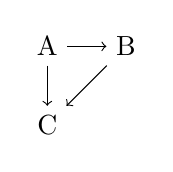
\begin{tikzpicture}
  \graph{A -> B; A -> C; B -> C};
\end{tikzpicture}


\section*{A table}

\begin{tabular}{|c|c|}
  \hline&\\
  $p(A)p(B|A)p(C|B)$&\adjustbox{valign=m}{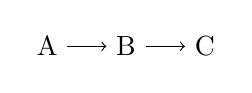
\begin{tikzpicture}\graph{A -> B -> C};\end{tikzpicture}}\\
  &\\\hline&\\
  $p(C)p(B|C)p(A|B)$&\adjustbox{valign=m}{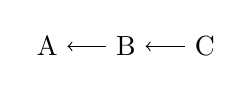
\begin{tikzpicture}\graph{A <- B <- C};\end{tikzpicture}}\\
  &\\\hline&\\
  $p(B)p(A|B)p(C|B)$&\adjustbox{valign=m}{\begin{tikzpicture}\graph{B -> A, B -> C};\end{tikzpicture}}\\
  &\\\hline
\end{tabular}

\end{document}
